\subsubsection{Theoretical Models}\label{sec_theoretical}

These models refine the Conceptual Models (Section~\ref{sec_conceptual}) using
natural language to improve their precision. This is a necessary step for
reducing ambiguity by explicitly stating how the primary sources are understood
and showing how they relate to the mathematically-defined Data Types
(Section~\ref{sec_typedefs}) and Instance Models (Section~\ref{sec_instance})
using Assumptions (Section~\ref{sec_assumptions}).

~\newline\noindent
\begin{minipage}{\textwidth}
    \renewcommand*{\arraystretch}{1.5}
    \begin{tabular}{| p{\colAwidth}  p{\colBwidth}|}
        \hline
        \colourRow
        \bf T\refstepcounter{theorynum}\thetheorynum
        \label{T_CalculateEmotionGP} &
        \bf Evaluate Emotion Kind from Goals and Plans \\
        \hline
    \end{tabular}
\end{minipage}

\paragraph{Description} The emotion kinds (``modes'') that CTE defines
(\cref{C_Appraisal-CTE}) that overlap with PES
(\aref{A_CTE2PES})---\textit{Happiness}, \textit{Sadness}, \textit{Fear},
\textit{Anger}, \textit{Disgust}---in terms of goals (\cref{C_Goals}) and plans
(\cref{C_Plans}) can be re-conceptualized as:
\begin{itemize}
    \item \textit{Joy} (\textit{Happiness}) occurs when an event transitions
    the previous world state to the current world state such that there is a
    change in the distance to a goal state where there is less distance between
    it and the current world state compared to the distance between it and the
    previous world state (i.e. a ``sub-goal'' of the goal, \aref{A_Subgoal})

    \item \textit{Sadness} occurs when an event transitions the previous world
    state to the current world state such that there is an unreachable plan
    state, implying that the plan is no longer viable, or when the distance
    from the current world state to a goal state is insurmountably large,
    implying that it is not possible to reach that goal state (i.e. ``lost'')

    \item \textit{Fear} (\textit{Anxiety}) occurs when a potential event
    transitions the current world state to a future world state where the
    distance between the future world state and a goal state is larger than the
    distance from the current world state and a goal state for a goal of type
    ``Self-Preservation'' OR it is impossible to satisfy the desired states of
    two different goals

    \item \textit{Anger} occurs when an event transitions the previous world
    state into the current world state that is not part of the entity's plan,
    but there is a series of events that transitions the current world state to
    another state that makes progress in the entity's plan

    \item \textit{Disgust} occurs when an event transitions the previous world
    state, where the entity's gustatory goal was satisfied, to the current
    world state that dissatisfies the goal such that the distance between the
    goal state and the current world state is larger than the distance to the
    previous world state
\end{itemize}

If an event elicits multiple emotions (\aref{A_Goal2Emotion}), they all
contribute to a single emotion state (\aref{A_OneState}).

Emotion intensity is evaluated separately (\aref{A_EmotionTypeIntensity}, see
\tref{T_CalculateEmotionIntensity}). The emotions \textit{Surprise},
\textit{Interest}, and \textit{Acceptance} are evaluated differently because
they are not part of CTE's primary emotions (\aref{A_AppraisalProcess}, see
\tref{T_CalculateEmotionSurprise}, \tref{T_CalculateEmotionInterest}, and
\tref{T_CalculateEmotionAcceptance} respectively). \\\hrule

\paragraph{Sources} --

\paragraph{Depends On} \aref{A_Subgoal}, \aref{A_Goal2Emotion},
\aref{A_OneState}, \aref{A_EmotionTypeIntensity}, \aref{A_AppraisalProcess},
\aref{A_CTE2PES}, \cref{C_Appraisal-CTE}, \cref{C_Goals}, \cref{C_Plans}

\paragraph{Ref. By} \tyref{TY_Goal}, \iref{IM_ElicitJoy},
\iref{IM_ElicitSadness}, \iref{IM_ElicitFear}, \iref{IM_ElicitAnger},
\iref{IM_ElicitDisgust}, \iref{IM_JoyIntensity}, \iref{IM_SadnessIntensity},
\iref{IM_FearIntensity}, \iref{IM_AngerIntensity}, \iref{IM_DisgustIntensity}
\\\hrule\vspace{0.5mm}\hrule

~\newpage\noindent
\begin{minipage}{\textwidth}
    \renewcommand*{\arraystretch}{1.5}
    \begin{tabular}{| p{\colAwidth}  p{\colBwidth}|}
        \hline
        \colourRow
        \bf T\refstepcounter{theorynum}\thetheorynum
        \label{T_CalculateEmotionIntensity} &
        \bf Evaluate Emotion Intensity (CTE) \\
        \hline
    \end{tabular}
\end{minipage}

\paragraph{Description} Of the four identified factors of emotion intensity
(\cref{C_EmIntensity-CTE}), only the value of the internal condition and the
event are within \progname{}'s scope. Users can extend \progname{}'s intensity
evaluations by integrating contextual considerations and/or personality
attributes to the evaluation after getting the initial evaluation.

Emotion intensity is proportional to the force causing an emotion state
(``entrained'') and how fixed or non-adjustable that force is (``locked in'').
From this, \progname{} assumes that emotion intensity directly relates to the
degree that something impacts a goal or plan such that an entity would want to
maintain the momentum caused by an emotion ``mode'' as long as that goal and/or
plan is affected (\aref{A_Goal2Intensity}). This aligns with the idea of an
affected ``internal condition''. \\\hrule

\paragraph{Sources} --

\paragraph{Depends On} \aref{A_Goal2Intensity}, \cref{C_EmIntensity-CTE}

\paragraph{Ref. By} \tyref{TY_EmotionIntensity}, \iref{IM_JoyIntensity},
\iref{IM_SadnessIntensity}, \iref{IM_FearIntensity}, \iref{IM_AngerIntensity},
\iref{IM_DisgustIntensity} \\\hrule\vspace{0.5mm}\hrule

~\newline

\noindent
\begin{minipage}{\textwidth}
    \renewcommand*{\arraystretch}{1.5}
    \begin{tabular}{| p{\colAwidth}  p{\colBwidth}|}
        \hline
        \colourRow
        \bf T\refstepcounter{theorynum}\thetheorynum
        \label{T_CalculateEmotionAcceptance} &
        \bf Evaluate \textit{Acceptance} Elicitation and Intensity \\
        \hline
    \end{tabular}
\end{minipage}

\paragraph{Description} CTE define ``emotions of attachment'' as an example of
infant-level social emotions, linking them to the ``basic'' emotion
\textit{Happiness}. Therefore, \progname{} takes the proposal that Trust is
\textit{Happiness} elaborated with information about social attachment
(\aref{A_Acceptance}).

Taking \textit{Acceptance} as a ``complex'' emotion
(\cref{C_ComplexEmotions-CTE}), it can be defined as \textit{Joy}
(\textit{Happiness}) elaborated with information about social relationships
(\cref{C_Relation-CTE}) such that an entity experiences \textit{Acceptance}
when \textit{an event transitions the previous world state to the current world
state such that there is a change in the distance to a goal state where there
is less distance between it and the current world state compared to the
distance between it and the previous world state AND a socially-relevant entity
caused the event}. An entity might also establish a relationship with another
entity that is attributed with causing the state, which would also elicit
\textit{Acceptance}.

For intensity, this implies that it is proportional to the intensity of
\textit{Joy} and the strength of the relationship with the entity that the
state is attributed to. \\\hrule

\paragraph{Sources} \citet[p.~178--179, 192]{oatley1992best}

\paragraph{Depends On} \aref{A_Acceptance}, \cref{C_ComplexEmotions-CTE},
\cref{C_Relation-CTE}

\paragraph{Ref. By} \tyref{TY_EmotionIntensity},
\iref{IM_CalculateEmotionAcceptanceElicit},
\iref{IM_CalculateEmotionAcceptance} \\\hrule\vspace{0.5mm}\hrule

~\newline

\clearpage\noindent
\begin{minipage}{\textwidth}
    \renewcommand*{\arraystretch}{1.5}
    \begin{tabular}{| p{\colAwidth}  p{\colBwidth}|}
        \hline
        \colourRow
        \bf T\refstepcounter{theorynum}\thetheorynum
        \label{T_CalculateEmotionInterest} &
        \bf Evaluate \textit{Interest} Elicitation and Intensity \\
        \hline
    \end{tabular}
\end{minipage}

\paragraph{Description} ``Sustained attention to certain external events''
(\cref{C_EmOther}) implies that it occurs when an entity is focused on the same
thing (e.g. task, another entity) for an extended period of time
(\aref{A_Interest}). From this, and ignoring the implied limitation to
events, \progname{} conceives \textit{Interest} as an evaluation where:
\textit{a significant amount of attention is paid to something}. This suggests
that there is a ``baseline'' amount of attention/time paid to something before
it triggers \textit{Interest}, which can differ between foci.

For intensity, this implies that it is proportional to the amount of time spent
focused on the same thing and relative to the ``baseline'' time spent. \\\hrule

\paragraph{Sources} --

\paragraph{Depends On} \aref{A_Interest}, \cref{C_EmOther}

\paragraph{Ref. By} \tyref{TY_EmotionIntensity},
\iref{IM_CalculateEmotionInterestElicit}, \iref{IM_CalculateEmotionInterest}
\\\hrule\vspace{0.5mm}\hrule

~\newline

\noindent
\begin{minipage}{\textwidth}
    \renewcommand*{\arraystretch}{1.5}
    \begin{tabular}{| p{\colAwidth}  p{\colBwidth}|}
        \hline
        \colourRow
        \bf T\refstepcounter{theorynum}\thetheorynum
        \label{T_CalculateEmotionSurprise} &
        \bf Evaluate \textit{Surprise} Elicitation and Intensity \\
        \hline
    \end{tabular}
\end{minipage}

\paragraph{Description} The description of \textit{Surprise} (\cref{C_EmOther})
needs clarification about what is meant by a ``sudden unexpected'' event.
Researchers have proposed that events appraised to be a contradiction of
explicitly or implicitly held expectations and beliefs elicit
\textit{Surprise}, which lab-based experiments found convincing supporting
evidence. Quantitative models of \textit{Surprise} intensity rely on event
probabilities such that an ``unexpected'' event is an improbable one, and
assume that intensity increases monotonically with the degree of
unexpectedness. This has no obvious conflicts with CTE's concept of emotions as
system-wide nonpropositional communication signals, EMgine conceives Surprise
as an evaluation where \textit{a significantly-improbable event happens}
(\aref{A_Surprise}). \\\hrule

\paragraph{Sources} \cite{reisenzein2019cognitive}

\paragraph{Depends On} \aref{A_Surprise}, \cref{C_EmOther}

\paragraph{Ref. By} \tyref{TY_EmotionIntensity},
\iref{IM_CalculateEmotionSurpriseElicit}, \iref{IM_CalculateEmotionSurprise}
\\\hrule\vspace{0.5mm}\hrule

~\clearpage

\noindent
\begin{minipage}{\textwidth}
    \renewcommand*{\arraystretch}{1.5}
    \begin{tabular}{| p{\colAwidth}  p{\colBwidth}|}
        \hline
        \colourRow
        \bf T\refstepcounter{theorynum}\thetheorynum
        \label{T_DecayEmotionState} &
        \bf Decaying Emotion State \\
        \hline
    \end{tabular}
\end{minipage}

\paragraph{Description} Emotion decay (\cref{C_EmDecay}) is a function of time
such that the emotion state returns to its ``equilibrium'' intensities as time
progresses. It is assumed that:
\begin{itemize}
    \item The speed that intensities return to ``equilibrium'' are assumed to
    be functions of distance such that larger differences between an intensity
    and its ``equilibrium'' cause larger changes in intensity
    (\aref{A_DecaySpeed})

    \item Each emotion kind has its own ``equilibrium'' value
    (\aref{A_Equilibrium}) and can decay at different rates
    (\aref{A_DecayRate}), allowing entities to vary the length of time it takes
    for them to return to ``normal'' variations between emotion kinds (e.g. if
    they experience \textit{Joy} they might extend that state by prolonging the
    decay to ``equilibrium'')

    \item Decay rates and equilibrium values can differ between entities
    (\aref{A_DecayUnique})
\end{itemize}
\hrule

\paragraph{Sources} --

\paragraph{Depends On} \aref{A_DecaySpeed}, \aref{A_Equilibrium},
\aref{A_DecayRate}, \aref{A_DecayUnique}, \cref{C_EmDecay}

\paragraph{Ref. By} \tyref{TY_EmotionDecay}, \tyref{TY_EmotionDecayState},
\iref{IM_DecayEmotionIntensity} \\\hrule\vspace{0.5mm}\hrule

~\newline

\noindent
\begin{minipage}{\textwidth}
    \renewcommand*{\arraystretch}{1.5}
    \begin{tabular}{| p{\colAwidth}  p{\colBwidth}|}
        \hline
        \colourRow
        \bf T\refstepcounter{theorynum}\thetheorynum
        \label{T_GetEmotionStatePAD} &
        \bf Getting an Emotion State as a PAD Point \\
        \hline
    \end{tabular}
\end{minipage}

\paragraph{Description} Assuming that an entity can only occupy one point in
PAD Space at any given time (\aref{A_OnePADPoint}), the intensities for each
discrete emotion in an emotion state must be combined into a single value for
each dimension in the space. However, there is no direct mapping between these
spaces. \progname{} must define reference points in PAD Space for each emotion
kind in the PES structure (\cref{C_EmotionStruct}), effectively ``mapping'' them
to PAD points. \progname{}'s approach for this heavily relies on the comparison
of emotion terms in each model for equal or comparable semantic meaning, which
is both subjective and error-prone. Unfortunately, there does not appear to be
a more reliable alternative.

From Plutchik's list of emotion terms and angular
placements~\citep[p.~170]{robert1980emotion}, assumed to have identical or
nearly identical meanings to PAD terms (\aref{A_EmotionTerms}), \progname{}
defines eight ``boundaries'' around circumplex areas for each of its emotion
kinds. ``Boundary'' terms are those where the perceived qualitative meaning
changes between it and the next listed term (Table~\ref{tab:pes-area},
Figure~\ref{fig:PESAreas}). For example, the change from ``Attentive'' to
``Joyful'' distinguishes a ``boundary'' between the \textit{Interest} and
\textit{Joy} areas because they do not ``feel'' like they have the same
qualitative meaning (i.e. ``Joyful'' implies a higher degree of pleasantness
than ``Attentive'', which does not imply either pleasantness or
unpleasantness). This mimics the idea of discrete emotion ``families'' such
that \progname{} can use one affective term to specify a PAD Space reference
point to serve as the emotion ``family'''s dimensional representation
(Figure~\ref{fig:theoryResolution}). Gaps between ``boundary'' terms are
inevitable due to the discrete nature of angular placements. However, they are
relatively small (between 0.3\textdegree{} and 7.3\textdegree{}), so
\progname{} ignored them instead of trying to compensate for them to avoid
introducing additional ``translation errors''.

\progname{} compiled eight lists---one for each derived circumplex
``area''---of exact or nearly exact matches of emotion terms in Plutchik and
PAD Space (Table~\ref{tab:pes-pad-terms}). \progname{} takes a single term from
each list as its PAD Space reference point for that Plutchik emotion, giving
preference to PAD terms that have statistically significant means ($p < 0.01$)
for each dimension, then to semantically equivalent terms. If there was no term
equivalence, \progname{} took the term closest to the midpoint of the Plutchik
circumplex ``area''. \progname{} ignores number of ratings and standard
deviation of PAD terms for simplicity (\aref{A_PADStats}). All terms achieved
significance for \textit{pleasure} and \textit{arousal}. \textit{Interested}
and \textit{Disgust} are not statistically significant for \textit{dominance}.

An emotion term's \textit{pleasure}, \textit{arousal}, and \textit{dominance}
mean values (\cref{C_PAD}) form a reference point. Number of ratings and
standard deviation do not affect reference points.

\begin{table}[H]
    \centering
    \renewcommand{\arraystretch}{1.2}
    \begin{tabular}{ccccc}
        \toprule
        \multicolumn{2}{c}{\textbf{PES}} &  &  & \\
        $k \in \emotionkindstype$ & Range on Circumplex (\textdegree) & Term  &
        Circumplex Location (\textdegree) & PAD Ref.~\# \\
        \midrule

        \colourRow\textit{Fear} & $[65.0, 86.0]$ & Terrified & 75.5 & 102 \\

        \textit{Anger} & $[200.6, 249.0]$ & Angry & 212.0 & 82 \\

        \colourRow\textit{Sadness} & $[88.3, 138.0]$ & Sad & 108.5 & 151 \\

        \textit{Joy} & $[323.4, 338.3]$ & Joyful & 323.4 & 20 \\

        \colourRow\textit{Interest} & $[249.7, 322.4]$ & Interested & 315.7 & 8
        \\

        \textit{Surprise} & $[138.3, 156.7]$ & Astonished & 148.0 & 74 \\

        \colourRow\textit{Disgust} & $[160.3, 193.7]$ & Disgusted & 161.3 & 75
        \\

        \textit{Acceptance} & $[340.7, 57.7]$ & Affectionate & 52.3 & 34 \\

        \bottomrule
    \end{tabular}
\end{table}

\hrule

\paragraph{Sources} \citet[p.~40, 42--45]{mehrabian1980basic},
\citet[p.~159, 170]{robert1980emotion}

\paragraph{Depends On} \aref{A_OnePADPoint}, \aref{A_EmotionTerms},
\aref{A_PADStats}, \cref{C_EmotionStruct}, \cref{C_PAD}

\paragraph{Ref. By} \iref{IM_GetEmotionStatePAD} \\\hrule\vspace{0.5mm}\hrule

\begin{table}[!ht]
    \renewcommand{\arraystretch}{1.2}
    \centering
    \caption{Summary of \progname{}-defined Areas on the PES Circumplex
        Structure based on Plutchik's Empirical Data}
    \label{tab:pes-area}
    \begin{tabular}{C{0.17\linewidth} C{0.18\linewidth} C{0.15\linewidth}}
        \toprule
        \textbf{Label} & \textbf{Range (\textdegree)} & \textbf{Midpoint
            (\textdegree)} \\ \midrule

        \colourRow\textit{Acceptance} & [340.7, 57.7] & 19.20 \\

        \textit{Fear} & [65.0, 86.0] & 75.50 \\

        \colourRow \textit{Sadness} & [88.3, 138.0] & 113.15 \\

        \textit{Surprise} & [138.3, 156.7] & 147.50 \\

        \colourRow \textit{Disgust} & [160.3, 193.7] & 177.00 \\

        \textit{Anger} & [200.6, 262.0] & 231.30 \\

        \colourRow \textit{Interest} & [249.7, 322.4] & 286.05 \\

        \textit{Joy} & [323.4, 338.3] & 330.85 \\

        \midrule\bottomrule
    \end{tabular}
\end{table}

\afterpage{
    \vspace*{\fill}
    \begin{figure}[!ht]
        \centering
        \includegraphics[width=0.7\linewidth]{figures/PESAreas.eps}

        \caption[\progname{}-Specific Emotion Kind Boundaries
        Circumplex]{\progname{}-Specific Emotion Kind Boundaries on the PES
            Circumplex Structure based on Plutchik's Empirical Data}
        \label{fig:PESAreas}
    \end{figure}

    \vspace*{\fill}

    \begin{figure}[!ht]
        \centering
        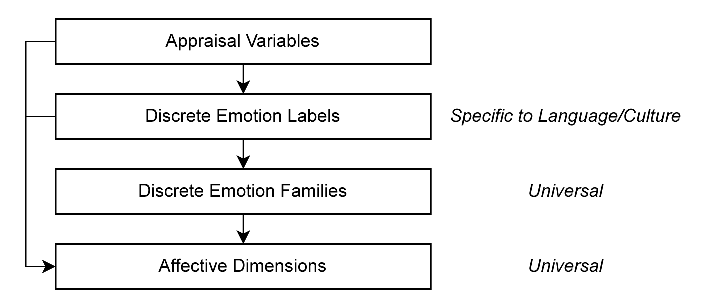
\includegraphics[width=0.65\linewidth]{figures/dataResolution.eps}

        \caption[Mapping Data Between Perspectives]{Mapping Data Between
            Perspectives, Adapted from \citet[p.~15]{scherer2010emotion}}
        \label{fig:theoryResolution}
    \end{figure}
    \vspace*{\fill}
}

\afterpage{\clearpage
    {\topskip0pt
        \vspace*{\fill}
        \begin{table}[!ht]
            \renewcommand{\arraystretch}{1.2}
            \centering
            \caption{Emotion Terms in Both PES and PAD Space with their
            Associated Empirical Data from Each}
            \label{tab:pes-pad-terms}
            \footnotesize
            \begin{tabular}{llc|lcccccccc}
                \toprule
                \multicolumn{3}{c|}{\textbf{Plutchik}} &
                \multicolumn{9}{c}{\textbf{PAD Space}} \\

                &  &  &  &  & & \multicolumn{2}{c}{\textbf{P}} &
                \multicolumn{2}{c}{\textbf{A}} & \multicolumn{2}{c}{\textbf{D}}
                \\

                \textbf{Area} & \textbf{Term} & \textbf{Angle} & \textbf{Term}
                & \textbf{\#} & \textbf{N} & \textbf{Mean} & \textbf{SD} &
                \textbf{Mean} & \textbf{SD} & \textbf{Mean} & \textbf{SD} \\
                \midrule

                \multirow{2}{*}{\begin{tabular}[x]{@{}l@{}}\textit{Accept-} \\
                        \textit{ance} \end{tabular}} & \colourCell
                {\footnotesize\textpmhg{\Hi}}Affectionate &
                \colourCell 52.3\textdegree & \colourCell Affectionate &
                \colourCell 34 & \colourCell 29 & \colourCell 0.64* &
                \colourCell 0.26 & \colourCell 0.35* & \colourCell 0.34 &
                \colourCell 0.24* & \colourCell 0.40 \\

                & Cooperative & 340.7\textdegree & Cooperative & 43 & 31 &
                0.39* & 0.32 & 0.13* & 0.27 & 0.03 & 0.34 \\

                \midrule

                \multirow{7}{*}{\textit{Fear}} & \colourCell Anxious &
                \colourCell 78.3\textdegree & \colourCell Anxious &
                \colourCell 50 & \colourCell 28 & \colourCell 0.01 &
                \colourCell 0.45 & \colourCell 0.59* & \colourCell 0.31 &
                \colourCell -0.15 & \colourCell 0.32 \\

                & Humiliated & 84.0\textdegree & Humiliated & 99 & 27 & -0.63*
                & 0.18 & 0.43* & 0.34 & -0.38* & 0.30 \\

                & \colourCell {\footnotesize\textpmhg{\Hi}}Terrified &
                \colourCell 75.7\textdegree & \colourCell Terrified &
                \colourCell 102 & \colourCell 29 & \colourCell -0.62* &
                \colourCell 0.20 & \colourCell 0.82* & \colourCell 0.25 &
                \colourCell -0.43* & \colourCell 0.34 \\

                & Helpless & 80.0\textdegree & Helpless & 104 & 29 & -0.71* &
                0.18 & 0.42* & 0.45 & -0.51* & 0.32 \\

                & \colourCell Embarrassed & \colourCell 75.3\textdegree &
                \colourCell Embarrassed & \colourCell 110 & \colourCell 29 &
                \colourCell -0.46* & \colourCell 0.30 & \colourCell 0.54* &
                \colourCell 0.26 & \colourCell -0.24* & \colourCell 0.40 \\

                & Shy & 72.0\textdegree & Shy & 117 & 29 & -0.15 & 0.33 & 0.06
                & 0.30 & -0.34* & 0.28 \\

                & \colourCell Timid & \colourCell 65.0\textdegree &
                \colourCell Timid & \colourCell 131 & \colourCell 28 &
                \colourCell -0.15 & \colourCell 0.41 & \colourCell -0.12 &
                \colourCell 0.37 & \colourCell -0.47* & \colourCell 0.31 \\

                \midrule

                \multirow{12}{*}{\textit{Sadness}} & Gloomy & 132.7\textdegree
                & Solemn & 72 & 29 & 0.03 & 0.39 & -0.32* & 0.26 & -0.11 & 0.33
                \\

                & \colourCell \begin{tabular}[x]{@{}l@{}} Grief- \\ Stricken
                \end{tabular} & \colourCell 127.3\textdegree &
                \colourCell Anguished & \colourCell 107 &
                \colourCell 29 & \colourCell -0.50* & \colourCell 0.30 &
                \colourCell 0.08 & \colourCell 0.46 & \colourCell -0.20* &
                \colourCell 0.34 \\

                & Guilty & 102.3\textdegree & Guilty & 118 & 29 & -0.57* & 0.19
                & 0.28* & 0.38 & -0.34* & 0.28 \\

                & \colourCell Remorseful & \colourCell 123.3\textdegree &
                \colourCell Regretful & \colourCell 123 & \colourCell 30 &
                \colourCell -0.52* & \colourCell 0.24 & \colourCell 0.02 &
                \colourCell 0.32 & \colourCell -0.21* & \colourCell 0.28 \\

                & Depressed & 125.3\textdegree & Depressed & 126 & 27 & -0.72*
                & 0.21 & -0.29* & 0.44 & -0.41* & 0.28 \\

                & \colourCell Despairing & \colourCell 133.0\textdegree &
                \colourCell Despairing & \colourCell 127 & \colourCell 27 &
                \colourCell -0.72* & \colourCell 0.21 & \colourCell -0.16 &
                \colourCell 0.34 & \colourCell -0.38* & \colourCell 0.25 \\

                & Lonely & 88.3\textdegree & Lonely & 128 & 29 & -0.66* & 0.35
                & -0.43* & 0.36 & -0.32* & 0.30 \\

                & \colourCell Meek & \colourCell 91.0\textdegree &
                \colourCell Meek & \colourCell 129 & \colourCell 29 &
                \colourCell -0.19 & \colourCell 0.58 & \colourCell -0.25* &
                \colourCell 0.32 & \colourCell -0.41* & \colourCell 0.42 \\

                & Bored & 136.0\textdegree & Bored & 132 & 28 & -0.65* & 0.19 &
                -0.62* & 0.24 & -0.33* & 0.21 \\

                & \colourCell Rejected & \colourCell 136.0\textdegree &
                \colourCell Rejected & \colourCell 137 & \colourCell 29 &
                \colourCell -0.62* & \colourCell 0.24 & \colourCell -0.01 &
                \colourCell 0.38 & \colourCell -0.33* & \colourCell 0.27 \\

                & Discouraged & 138.0\textdegree & Discouraged & 150 & 30 &
                -0.61* & 0.25 & -0.15 & 0.32 & -0.29* & 0.32 \\

                & \colourCell {\footnotesize\textpmhg{\Hi}}Sad &
                \colourCell 108.5\textdegree & \colourCell Sad &
                \colourCell 151 & \colourCell 30 & \colourCell -0.63* &
                \colourCell 0.23 & \colourCell -0.27* & \colourCell 0.34 &
                \colourCell -0.33* & \colourCell 0.22 \\

                \midrule

                \multirow{4}{*}{\textit{Surprise}} & Surprised &
                146.7\textdegree & Surprised & 52 & 29 & 0.40* & 0.30 & 0.67* &
                0.27 & -0.13 & 0.38 \\

                & \colourCell Awed & \colourCell 156.7\textdegree &
                \colourCell Awed & \colourCell 56 & \colourCell 30 &
                \colourCell 0.18* & \colourCell 0.34 & \colourCell 0.40* &
                \colourCell 0.30 & \colourCell -0.38* & \colourCell 0.21 \\

                & {\footnotesize\textpmhg{\Hi}}Astonished & 148.0\textdegree &
                Astonished & 74 & 30 & 0.16* & 0.26 & 0.88* & 0.19 & -0.15* &
                0.26 \\

                & \colourCell Confused & \colourCell 141.3\textdegree &
                \colourCell Confused & \colourCell 121 & \colourCell 30 &
                \colourCell -0.53* & \colourCell 0.20 & \colourCell 0.27* &
                \colourCell 0.29 & \colourCell -0.32* & \colourCell 0.28 \\

                \midrule

                \multirow{7}{*}{\textit{Disgust}} &
                {\footnotesize\textpmhg{\Hi}}Disgusted & 161.3\textdegree &
                Disgusted & 75 & 29 & -0.60* & 0.20 & 0.35* & 0.41 & 0.11 &
                0.34 \\

                & \colourCell \begin{tabular}[x]{@{}l@{}} Contempt- \\ uous
                \end{tabular} & \colourCell 192.0\textdegree &
                \colourCell Contempt & \colourCell 85 & \colourCell 29 &
                \colourCell -0.23* & \colourCell 0.39 & \colourCell 0.31* &
                \colourCell 0.33 & \colourCell 0.18* & \colourCell 0.29 \\

                & Suspicious & 182.7\textdegree & Suspicious & 90 & 29 & -0.25*
                & 0.23 & 0.42* & 0.21 & 0.11 & 0.32 \\

                & \colourCell Distrustful & \colourCell 185.0\textdegree &
                \colourCell Skeptical & \colourCell 91 & \colourCell 29 &
                \colourCell -0.22* & \colourCell 0.28 & \colourCell 0.21* &
                \colourCell 0.25 & \colourCell 0.03 & \colourCell 0.33 \\

                & Displeased & 181.5\textdegree & Displeased & 109 & 29 &
                -0.55* & 0.21 & 0.16 & 0.34 & -0.05 & 0.41 \\

                & \colourCell Indignant & \colourCell 175.0\textdegree &
                \colourCell \begin{tabular}[x]{@{}l@{}}Quietly \\ Indignant
                \end{tabular} & \colourCell 114 & \colourCell 26 &
                \colourCell -0.28* & \colourCell 0.35 & \colourCell 0.04 &
                \colourCell 0.36 & \colourCell -0.16 & \colourCell 0.40 \\

                & Dissatisfied & 183.0\textdegree & Dissatisfied & 122 & 30 &
                -0.50* & 0.22 & 0.05 & 0.28 & 0.13 & 0.32 \\

                \midrule\bottomrule
            \end{tabular}
        \end{table}
        \vspace*{\fill}}

    \clearpage

    {\topskip0pt
        \addtocounter{table}{-1}
        \captionsetup{list=no}
        \begin{table}[!hb]
            \renewcommand{\arraystretch}{1.2}
            \centering
            \caption{\textit{(Continued)} Emotion Terms in Both PES and PAD
            Space with their Associated Empirical Data from Each}
            \footnotesize
            \begin{threeparttable}
                \begin{tabular}{llc|lcccccccc}
                    \toprule
                    \multicolumn{3}{c|}{\textbf{Plutchik}} &
                    \multicolumn{9}{c}{\textbf{PAD Space}} \\

                    &  &  & & &  & \multicolumn{2}{c}{\textbf{P}} &
                    \multicolumn{2}{c}{\textbf{A}} &
                    \multicolumn{2}{c}{\textbf{D}} \\

                    \textbf{Area} & \textbf{Term} & \textbf{Angle} &
                    \textbf{Term} & \textbf{\#} & \textbf{N} & \textbf{Mean} &
                    \textbf{SD} & \textbf{Mean} & \textbf{SD} & \textbf{Mean} &
                    \textbf{SD} \\
                    \midrule

                    \multirow{8}{*}{\textit{Anger}} & \colourCell Aggressive &
                    \colourCell 232.0\textdegree & \colourCell Aggressive &
                    \colourCell 13 & \colourCell 28 & \colourCell 0.41* &
                    \colourCell 0.30 & \colourCell 0.63* & \colourCell 0.25 &
                    \colourCell 0.62* & \colourCell 0.24 \\

                    & Irritated & 202.3\textdegree & Irritated & 78 & 29 &
                    -0.58* & 0.16 & 0.40* & 0.37 & 0.01 & 0.40 \\

                    & \colourCell Defiant & \colourCell 230.7\textdegree &
                    \colourCell Defiant & \colourCell 79 & \colourCell 28 &
                    \colourCell -0.16* & \colourCell 0.30 & \colourCell 0.54* &
                    \colourCell 0.37 & \colourCell 0.32* & \colourCell 0.42 \\

                    & Hostile & 222.0\textdegree & Hostile & 81 & 29 & -0.42* &
                    0.31 & 0.53* & 0.36 & 0.30* & 0.32 \\

                    & \colourCell {\footnotesize\textpmhg{\Hi}}Angry &
                    \colourCell 212.0\textdegree & \colourCell Angry &
                    \colourCell 82 & \colourCell 29 & \colourCell -0.51* &
                    \colourCell 0.20 & \colourCell 0.59* & \colourCell 0.33 &
                    \colourCell 0.25* & \colourCell 0.39 \\

                    & Annoyed & 200.6\textdegree & Mildly Annoyed & 83 & 29 &
                    -0.28* & 0.16 & 0.17* & 0.28 & 0.04 & 0.31 \\

                    & \colourCell Furious & \colourCell 221.3\textdegree &
                    \colourCell Enraged & \colourCell 84 & \colourCell 29 &
                    \colourCell -0.44* & \colourCell 0.25 & \colourCell 0.72* &
                    \colourCell 0.29 & \colourCell 0.32* & \colourCell 0.44 \\

                    & Scornful & 227.0\textdegree & Scornful & 89 & 28 & -0.35*
                    & 0.21 & 0.35* & 0.27 & 0.29* & 0.32 \\

                    \midrule

                    \multirow{7}{*}{\textit{Interest}} &
                    \colourCell Adventurous & \colourCell 270.7\textdegree &
                    \colourCell Bold & \colourCell 1 & \colourCell 27 &
                    \colourCell 0.44* & \colourCell 0.32 & \colourCell 0.61* &
                    \colourCell 0.24 & \colourCell 0.66* & \colourCell 0.30 \\

                    & Proud & 262.0\textdegree & Proud & 7 & 29 & 0.77* & 0.21
                    & 0.38* & 0.34 & 0.65* & 0.33 \\

                    & \colourCell {\footnotesize\textpmhg{\Hi}}Interested &
                    \colourCell 315.7\textdegree & \colourCell Interested &
                    \colourCell 8 & \colourCell 29 & \colourCell 0.64* &
                    \colourCell 0.20 & \colourCell 0.51* & \colourCell 0.21 &
                    \colourCell 0.17 & \colourCell 0.40 \\

                    & Elated & 311.0\textdegree & Elated & 17 & 28 & 0.50* &
                    0.47 & 0.42* & 0.14 & 0.23* & 0.36 \\

                    & \colourCell Hopeful & \colourCell 298.0\textdegree &
                    \colourCell Hopeful & \colourCell 18 & \colourCell 29 &
                    \colourCell 0.51* & \colourCell 0.30 & \colourCell 0.23* &
                    \colourCell 0.33 & \colourCell 0.14 & \colourCell 0.41 \\

                    & Wondering & 249.7\textdegree & Wonder & 54 & 30 & 0.27* &
                    0.37 & 0.24* & 0.35 & -0.17* & 0.26 \\

                    & \colourCell Curious & \colourCell 261.0\textdegree &
                    \colourCell Curious & \colourCell 58 & \colourCell 28 &
                    \colourCell 0.22* & \colourCell 0.30 & \colourCell 0.62* &
                    \colourCell 0.20 & \colourCell -0.01 & \colourCell 0.34 \\

                    \midrule

                    \multirow{2}{*}{\textit{Joy}}&
                    {\footnotesize\textpmhg{\Hi}}Joyful & 323.4\textdegree &
                    Joyful & 20 & 29 & 0.76* & 0.22 & 0.48* & 0.26 & 0.35* &
                    0.31 \\

                    & \colourCell Happy & \colourCell 323.7\textdegree &
                    \colourCell Happy & \colourCell 31 & \colourCell 29 &
                    \colourCell 0.81* & \colourCell 0.21 & \colourCell 0.51* &
                    \colourCell 0.26 & \colourCell 0.46* & \colourCell 0.38 \\

                    \hline\bottomrule
                \end{tabular}
                \begin{tablenotes}

                    \footnotesize
                    \vspace*{2mm}

                    \item N \textit{Number of Ratings}

                    \item SD \textit{Standard Deviation}

                    \item {\normalsize*} \textit{Statistically Significant ($p
                        > 0.01$)}

                    \item {\small\textpmhg{\Hi}} \textit{Chosen term}

                \end{tablenotes}
            \end{threeparttable}%
        \end{table}
    }
    \captionsetup{list=yes}
}